%\documentclass[
  bibliography=totoc,     % Literatur im Inhaltsverzeichnis
  captions=tableheading,  % Tabellenüberschriften
  titlepage=firstiscover, % Titelseite ist Deckblatt
]{scrartcl}

% Paket float verbessern
\usepackage{scrhack}

% Warnung, falls nochmal kompiliert werden muss
\usepackage[aux]{rerunfilecheck}

% unverzichtbare Mathe-Befehle
\usepackage{amsmath}
% viele Mathe-Symbole
\usepackage{amssymb}
% Erweiterungen für amsmath
\usepackage{mathtools}

% Fonteinstellungen
\usepackage{fontspec}
% Latin Modern Fonts werden automatisch geladen
% Alternativ zum Beispiel:
%\setromanfont{Libertinus Serif}
%\setsansfont{Libertinus Sans}
%\setmonofont{Libertinus Mono}

% Wenn man andere Schriftarten gesetzt hat,
% sollte man das Seiten-Layout neu berechnen lassen
\recalctypearea{}

% deutsche Spracheinstellungen
\usepackage[ngerman]{babel}


\usepackage[
  math-style=ISO,    % ┐
  bold-style=ISO,    % │
  sans-style=italic, % │ ISO-Standard folgen
  nabla=upright,     % │
  partial=upright,   % │
  mathrm=sym,        % ┘
  warnings-off={           % ┐
    mathtools-colon,       % │ unnötige Warnungen ausschalten
    mathtools-overbracket, % │
  },                       % ┘
]{unicode-math}

% traditionelle Fonts für Mathematik
\setmathfont{Latin Modern Math}
% Alternativ zum Beispiel:
%\setmathfont{Libertinus Math}

\setmathfont{XITS Math}[range={scr, bfscr}]
\setmathfont{XITS Math}[range={cal, bfcal}, StylisticSet=1]

% Zahlen und Einheiten
\usepackage[
  locale=DE,                   % deutsche Einstellungen
  separate-uncertainty=true,   % immer Unsicherheit mit \pm
  per-mode=symbol-or-fraction, % / in inline math, fraction in display math
]{siunitx}

% chemische Formeln
\usepackage[
  version=4,
  math-greek=default, % ┐ mit unicode-math zusammenarbeiten
  text-greek=default, % ┘
]{mhchem}

% richtige Anführungszeichen
\usepackage[autostyle]{csquotes}

% schöne Brüche im Text
\usepackage{xfrac}

% Standardplatzierung für Floats einstellen
\usepackage{float}
\floatplacement{figure}{htbp}
\floatplacement{table}{htbp}

% Floats innerhalb einer Section halten
\usepackage[
  section, % Floats innerhalb der Section halten
  below,   % unterhalb der Section aber auf der selben Seite ist ok
]{placeins}

% Seite drehen für breite Tabellen: landscape Umgebung
\usepackage{pdflscape}

% Captions schöner machen.
\usepackage[
  labelfont=bf,        % Tabelle x: Abbildung y: ist jetzt fett
  font=small,          % Schrift etwas kleiner als Dokument
  width=0.9\textwidth, % maximale Breite einer Caption schmaler
]{caption}
% subfigure, subtable, subref
\usepackage{subcaption}

% Grafiken können eingebunden werden
\usepackage{graphicx}

% schöne Tabellen
\usepackage{tabularray}
\UseTblrLibrary{booktabs, siunitx}

% Verbesserungen am Schriftbild
\usepackage{microtype}

% Literaturverzeichnis
\usepackage[
  backend=biber,
]{biblatex}
% Quellendatenbank
\addbibresource{lit.bib}
\addbibresource{programme.bib}

% Hyperlinks im Dokument
\usepackage[
  german,
  unicode,        % Unicode in PDF-Attributen erlauben
  pdfusetitle,    % Titel, Autoren und Datum als PDF-Attribute
  pdfcreator={},  % ┐ PDF-Attribute säubern
  pdfproducer={}, % ┘
]{hyperref}
% erweiterte Bookmarks im PDF
\usepackage{bookmark}

% Trennung von Wörtern mit Strichen
\usepackage[shortcuts]{extdash}

\author{%
  Vincent Wirsdörfer\\%
  \href{mailto:vincent.wirsdoerfer@udo.edu}{authorA@udo.edu}%
  \and%
  Joris Daus\\%
  \href{mailto:joris.daus@udo.edu}{authorB@udo.edu}%
}
\publishers{TU Dortmund – Fakultät Physik}


%\begin{document}
\section{Diskussion}
\label{sec:Diskussion}
 
\subsection{Kennlinie}

Allgemein lassen sich alle Grundsätze der theoretischen Vorhersage empirisch bestätigen. Der grobe Verlauf aller gemessenen Kennlinien
entspricht dem in der Theorie postulierten logistischem Wachstum. Bei kleinen bis mittleren Spannungen steigt der Anodenstrom exponentiell
an, bevor die Kennlinie gegen den Sättigungsstrom konvergiert. Auch die Relationen der Kennlinien untereinander stimmen überein, da der Sättigungsstrom 
bei größer werdenden Heizströmen ebenfalls ansteigt.

\subsection{Raumladungsgesetz}

Auch das Langmuir-Schottkysche Raumladungsgesetz kann partiell durch den Versuch bestätigt werden. Mit einer Steigung von 
$m = 1.395\pm0.013$ ähnelt der Verlauf eher einem linearen Wachstum und erfüllt nur teilweise die $\sqrt{U³}$-Gesetzmäßigkeit.
Mögliche Ursachen für diesen Fehler könnten Parallaxenfehler sein, welche sich in einer signifikanten Fehlerbehaftung der Heizströme 
und Heizspannungen bemerkbar macht. Auch die Tatsache, dass sich einige Milliampere über die Messzeit gesammelt haben könnten und somit 
die Messergebnisse verfälschen könnten ist nicht auszuschließen.

\subsection{Anlaufstrom}

Die Untersuchung des Anlaufstromgebiets beinhaltet mit einer Kathodentemperatur von $T_\text{K} = \qty{2020\pm90}{\kelvin}$ einen ähnlich 
großen Fehler. Im Gegensatz zum Raumladungsgesetz bietet das Anlaufstromgebiet jedoch ein breites Spektrum an Fehlerpotential:
Der Anlaufstrom hat die intrinsische Eigenschaft sehr klein zu sein. Er befindet sich im \unit{\nano \ampere} Bereich. 
Dementsprechend reagiert das Strommessgerät bereits bei geringen Umwelteinflüssen sehr sensitiv. Tatsächlich ist es so empfindlich, dass es kleinste Störungen 
der Umgebung das Messergebnis beeinflussen. Während der Aufnahme der Messreihen kann beobachtet werden, dass selbst das 
bloße Halten der Hand neben der Hochvakuumdiode zu einer Veränderung des Stromausschlags führt. Dies kann auf eine statische 
Ladung der Hand zurückzuführen sein. Da die Elektronen aufgrund eines elektrischen Feldes zur Anode gezogen werden, kann das 
E-Feld der Hand somit die Messung beeinflussen. Andere Störfaktoren werden nicht ausgeschlossen. Aus diesem Grund werden 
möglichst wenig Messdaten mit geringem Strom gemessen, und mehr mit etwas höherem Strom. \\
\noindent Dessen ungeachtet entspricht der qualitative Verlauf der Anlaufspannung den theoretischen Erwartungen. Er fügt sich 
einem exponentiellen Verlauf, welcher für größer werdende Gegenspannungen zunimmt. \footnote{Da das Anlaufstromgebiet für 
negative Spannungen definiert wird, entspricht eine positive Gegenspannung einer negativen Spannung der Kennlinie} 


\subsection{Austrittsarbeit}

Der gemessene Mittelwert der Austrittsarbeit von Wolfram beträgt $\bar{E}_\text{A} = \qty{4.77\pm0.07}{\electronvolt}$. Im Vergleich dazu 
liegt der Literaturwert der Austrittsarbeit von Wolfram zwischen \qty{4.54}{\electronvolt} und \qty{4.60}{\electronvolt}\cite{Austrittsarbeit}.
Dies bedeutet konkret eine prozentuale Abweichung $\increment{}E_\text{A} \approx \qty{4.38}{\percent}$. Diese Abweichung zeigt bereits, dass augenscheinlich keine 
markanten systematischen Fehler die Messung beeinträchtigen. Effektiv hängt die Berechnung von der Kathodentemperatur und der Sättigungsstromdichte ab.
Neben den bereits thematisierten Fehlern des Heizstroms und der Heizspannung, schöpft der gemessene Wert der Austrittsarbeit somit möglicherweise 
auch ein Fehlerpotential durch einen inkorrekten Sättigungsstromwert. Dies ist durchaus realistisch, da gerade für höhere Heizströme noch keine 
eindeutige Konvergenz der Kennlinien konstatiert werden kann.

\section{Anhang}

\begin{figure}[H]
    \centering
    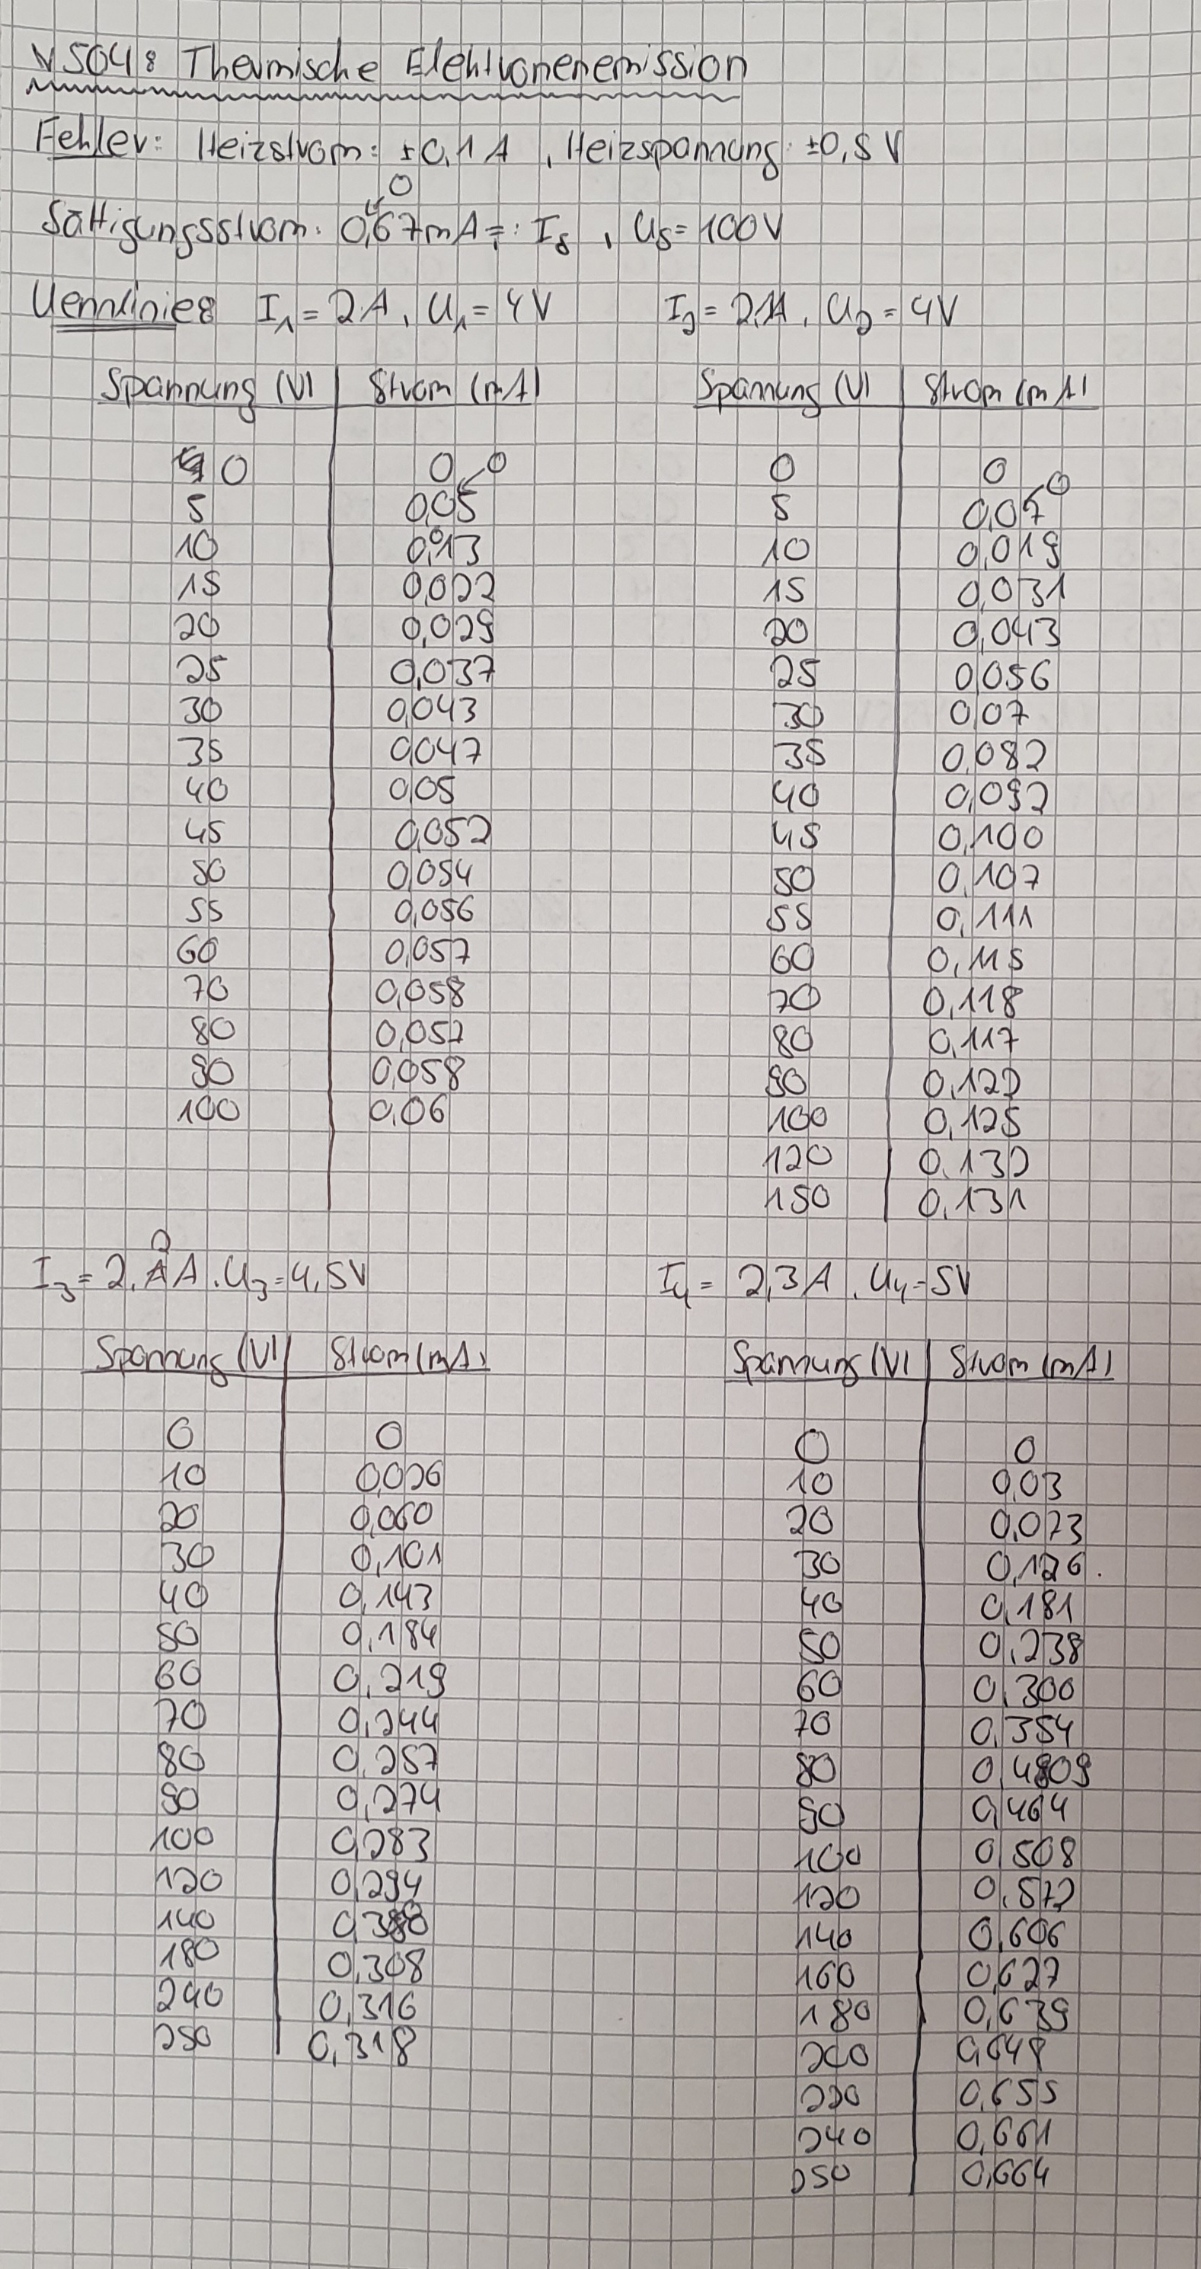
\includegraphics[height=0.9\textheight]{content/Laborbuch1.jpg}
    \caption{Laborbuch Seite 1.}
\end{figure}

\begin{figure}[H]
    \centering
    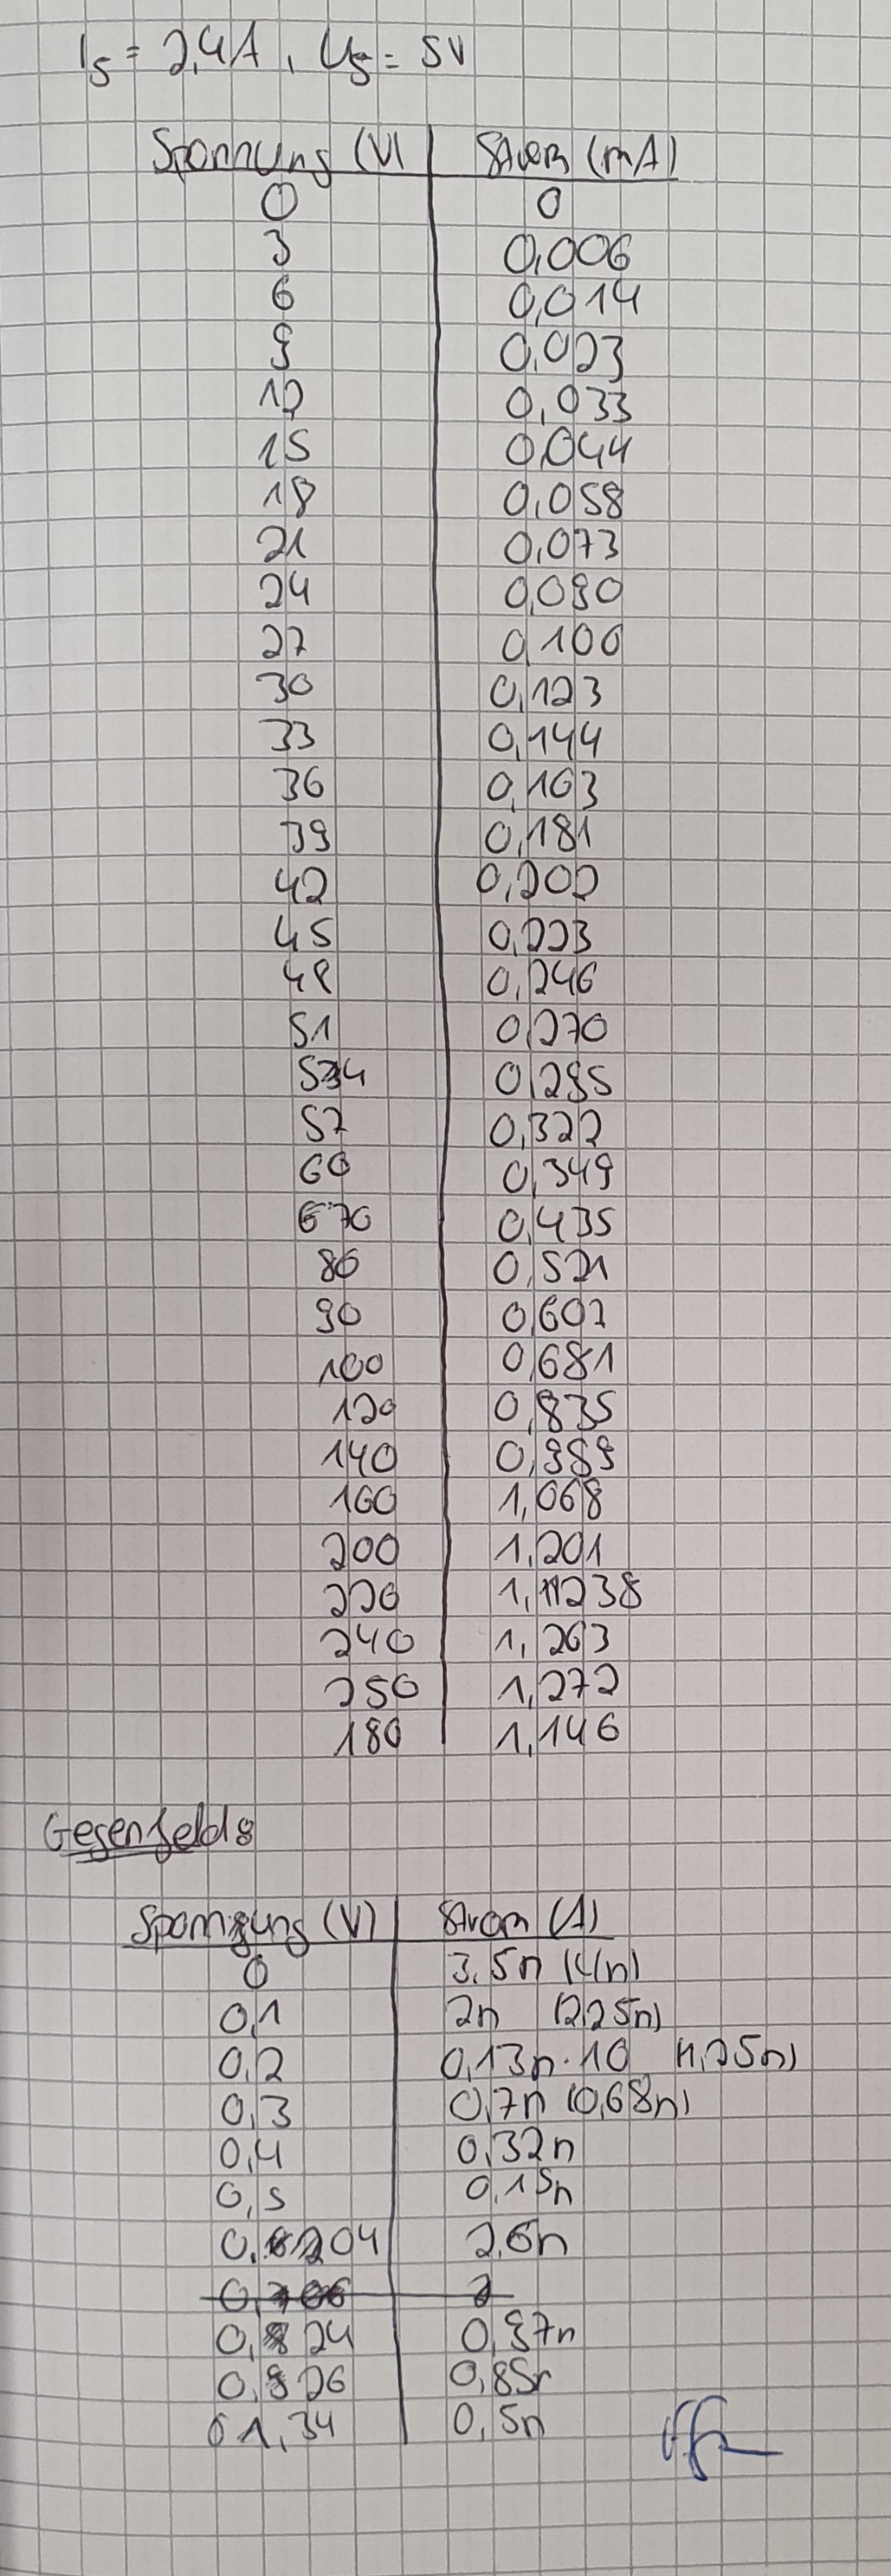
\includegraphics[height=0.9\textheight]{content/Laborbuch2.jpg}
    \caption{Laborbuch Seite 2.}
\end{figure}




%\end{document}
